\documentclass[a4paper,12pt]{article}
\usepackage[a4paper, margin=2.4cm]{geometry}
\usepackage[utf8]{inputenc}
\usepackage{amsmath, amssymb} % Packages pour les maths
\usepackage[T1]{fontenc}
\usepackage{graphicx} 
\usepackage{caption}
\usepackage{setspace} % Espacement des lignes
\usepackage{tikz}
\usepackage{titlesec}
\titleformat*{\section}{\LARGE\bfseries}
\titleformat*{\subsection}{\Large\bfseries}
\titleformat*{\subsubsection}{\normalsize\bfseries}
\begin{document}
\section*{Modèle 3: Avec intérieur de la coquille non vide }
\subsubsection*{Hypothèses:}
\begin{itemize}
    \item Terre assimilée à une coquille d'eau avec intérieur non vide 
    \item  conduction entre centre de la terre et croûte (\(P_r\))
    \item  conduction entre croûte et air (\(P_{th,cond}\))
    \item  rayonnement de la croûte (\(P_{th,ray}\))
    \item On néglige le rayonnement de l'atmosphère
    \item $T(t=0) = T_i$ \ \ \
$T(t \to +\infty) = T_0$
    
    
    
\end{itemize}

\subsubsection*{Schéma:} 
\noindent\textcolor{gray}{\rule{\linewidth}{0.4pt}}

    
\begin{center}
  \input{modele3/figures/Schéma modèle 3 coquille.txt}
\end{center}
\noindent\textcolor{gray}{\rule{\linewidth}{0.4pt}}

\subsubsection*{Équations de transfert thermique}

On applique le premier principe appliqué au système \{ Coquille non vide  \}
\[
(-P_{\mathrm{th,cond}} - P_{\mathrm{th,ray}} + P_r)\,dt = C\,dT.
\]

\[
-\,h\bigl[T(r+dr)-T_0\bigr]\;4\pi
\;-\;4\pi\,\cdot (r+dr)^2\,\sigma\,T^4(r+dr)
\;-\;4\pi\,r^2\,\lambda\,\frac{\partial T}{\partial r}(r)
\;=\;C\,\frac{dT}{dt}.
\]

\medskip

Or au \(1^{er}\) ordre en \(dr\), \(r+dr\approx r\) :

\[
-4\pi\,h\bigl(T(r)-T_0\bigr)
\;-\;4\pi\,r^2\,\sigma\,T(r)^4
\;-\;4\pi\,r^2\,\lambda\,\frac{\partial T}{\partial r}(r)
\;=\;C\,\frac{dT}{dt}.
\]

\medskip

Avec
\[
P_{r}
= \iint\vec j_{\mathrm{thr}}\cdot d\vec S
= \iint -\lambda\,\vec{ \nabla } T\cdot d\vec S
= -\lambda
  \int_{0}^{\pi}\!\!\int_{0}^{2\pi}
    \frac{\partial T}{\partial r}\,\vec e_{r}\,
    r^2\sin\theta\;d\theta\,d\varphi\;\vec e_{r}
= -\lambda\,4\pi\,r^2\,\frac{\partial T}{\partial r}.
\]

\textbf{Modélisation graphique :} 
    
    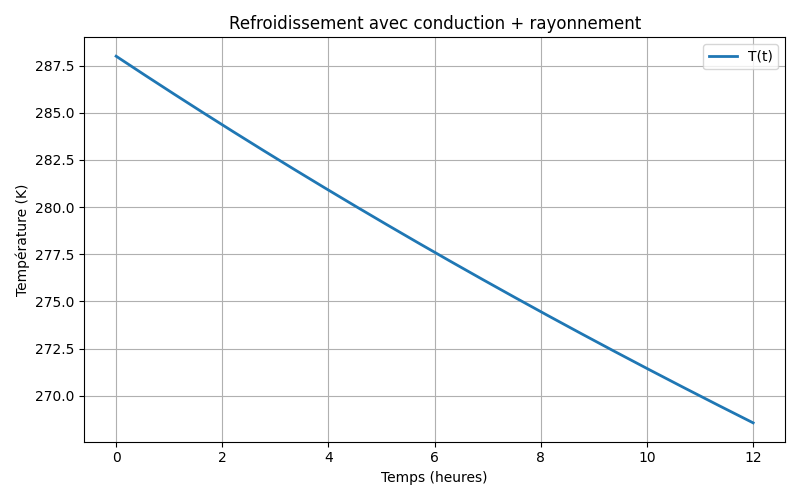
\includegraphics[width=0.8\linewidth]{../modele3/figures/modele3_coquille-conduction-rayonnement.png}    


\textbf{Critique du modèle}
\vspace{1cm}
\begin{itemize}
    \item La convection n’est pas prise en compte.
    \item dr doit être choisi de façons à ce que la température ne varie pas significativement.
    \item Problème de définition de $T_0$ :
    \begin{itemize}
        \item Si on suit notre modèle, ce serait la température au-delà de la thermosphère.
        \item Or on a posé $T_0 = 273\, \mathrm{K}$ dans nos codes Python. 
    
    \end{itemize}
\end{itemize}
\end{document}